\cut{
1. (way ahead of time) train a statistical model over the training data
2. (at inference time) coarse-grain tokenization (i.e. finding Seqsets)
3a. run the statistical model over the user data, and use the (modified) 
    viterbi algorithm to find the most likely sequences
3b. populate histograms based on the most likely sequences
3c. select candidate histograms + structure, according to heuristics
3d. break down Seqsets using not just the most likely sequences
3e. recursively repeat, go to 3a.
4. apply rewriting involving blob finding to maximize the information 
   theoretic complexity score

We'll compose this algorithm by figure and explain it with running examples 
in Section 2.
}

\section{Description Inference Algorithm}\label{sec:algo}

We propose a multi-phase algorithm to attack the problem of
format inference for ad hoc data. 
The main components of
this algorithm are {\em training of statistical model}, 
{\em probablistic tokenization} of raw data, 
a recursive {\em structure discovery} procedure,
and a {\em format refinement} phase. This is similar to 
the algorithm proposed in our earlier work \cite{fisher+:dirttoshovels}. 
The key difference is, instead of making definitive decisions about 
tokenization up front, we defer such decision well into the structure
discovery phase. In particular, we produce {\em all possible} token 
sequences for each data chunk and make choices among these possible 
sequences as the structure is being constructed in an incremental fashion.

%(3a) find the most probable token sequence for each chunk, and 
%     if that sequence of every chunk contains only 1 or 0 edges 
%     then return else go to (3b)
%(3b) construct histograms from the most probably sequences and 
%     predict a top-level structure;
%(3c) populate sub-components of the predicated structure with \seqset's
%     or sub-\seqset's;
%(3d) for each sub-component, recurse to (3a);

\begin{figure}[t]
\begin{centercode}
(1) Train a statistical model from the labeled training data;
(2) Tokenize the test data into \seqset's, one \seqset{} per chunk;
(3) Discover an initial structure of the data based on the \seqset's;
(4) Apply rewriting rules to improve the overall structure
\end{centercode}
\caption{High-level Inference Algorithm}\label{fig:algo}
\end{figure}

Fig. \ref{fig:algo} presents this high-level algorithm. We now explain
it step-by-step with the help of the {\tt yum.txt} example.
Because this algorithm shares the general structure and many details with
the original algorithm, we only highlight the differences and
refer the reader to \cite{fisher+:dirttoshovels} for complete discussion of
the original algorithm.

\subsection{Model training}
Well ahead of time, a statistical model is trained with
a large pool of sample data formats. Section \ref{sec:stats} has more details
about the various models we experimented with in this algorithm. To train the models,
we first label the data using a set of predefined tokens. The labeling
is done with a built-in tool that automatically labels all the tokens
given a \pads{} description of the data. The set of tokens
used are primarily system oriented, which include
integer, float, time, date, ip address, hostname, file path, URL, 
word, id, white space and punctuations. 
%A given substring may be parsed by more than one of the token
%types, and we pick a token that best represent the meaning of the data.
We assume that parsing of tokens is {\em greedy}, i.e.
each token matches the longest possible substring, hence
the string ``43.8'' can be parsed by sequences 
{\tt [int] [.] [int]}, {\tt [int] [.] [float]}, or {\tt [float]},
but not by {\tt [float] [.] [int]} or {\tt [float] [.] [float]},
because the token {\tt float} would parse the entire string, even though
the string ``43'' alone can be represented by a {\tt [float]}.

\subsection{Probablistic tokenization}
When the user tries to infer a description, each chunk of the data 
is parsed into the set of all possible token sequences. 
Because these sequences have
common subsequences, we organize them in a directed acyclic graph
called \seqset. Fig.\ref{fig:seqset} shows the \seqset{} after parsing 
the substring ``2.2.13-4'' from a chunk in Fig.\ref{fig:yum}. It 
forms a small part of the \seqset{} for the entire chunk.

\begin{figure}[th]
\begin{center}
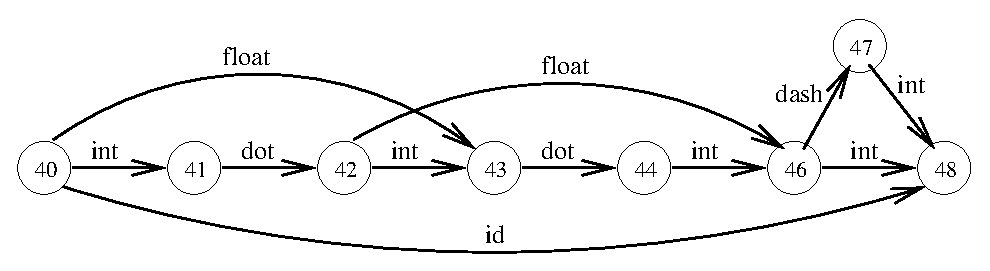
\epsfig{file=seqset.eps, width=0.9\columnwidth}
\end{center}
\caption{\seqset{} from parsing string ``2.2.13-4''}\label{fig:seqset}
\end{figure}

The edges of the \seqset{} are tokens and the vertices are the end locations
of the preceding token. If there is no preceding token (e.g. the leftmost
vertex of the entire \seqset), then the vertex is the begin location 
of first character of next token.
The construction of the \seqset, though expensive, is done only once.
The \seqset{} is used subsequently as input to the recursive 
structure discovery procedure and gets updated during each recursion.

\begin{figure}[t]
\begin{centercode}
type description (* an intermediate representation *)
type seqset       (* a seqset *)
type seqsets = seqset list

(* A top-level description guess *)
datatype prophecy =
   BaseProphecy   of description
 | StructProphecy of seqsets list 
 | ArrayProphecy  of seqsets * seqsets * seqsets
 | UnionProphecy  of seqsets list

(* Guesses the best top-level description *)
fun oracle : seqsets -> prophecy

(* Implements a generic inference algorithm *)
fun discover (sqs:seqsets) : description =
 case (oracle sqs) of
   BaseProphecy b => b

 | StructProphecy sqss => 
     let Ts = map discover sqss in
     struct \{ Ts \}

 | ArrayProphecy (sqsfirst,sqsbody,sqslast) => 
     let Tfirst = discover sqsfirst in
     let Tbody  = discover sqsbody  in
     let Tlast  = discover sqslast  in
     struct \{ Tfirst; array \{ Tbody \}; Tlast; \}

 | UnionProphecy sqss => 
     let Ts = map discover sqss in
     union \{ Ts \}
\end{centercode}
\caption{A generic structure-discovery algorithm in Pseudo-ML.} 
\label{fig:structure-discovery}
\end{figure}

\subsection{Structure discovery}
This is a {\em top-down}, {\em divide-and-conquer} algorithm outlined in
Fig.\ref{fig:structure-discovery} in pseudo-ML code. 
During each recursive call
of the function {\tt discover}, which is the main procedure in
this algorithm, an {\tt oracle} function is invoked to
make a ``magical'' guess about the structure of the data represented by
the current list of \seqset's. The structure can be 
either a {\em base type}, a {\em struct}, an {\em array} or a {\em union}.
The {\tt oracle} function also breaks up the input \seqset's into
sets of sub-\seqset's, each of which corresponds to a component in
the guessed structure.
After that, the procedure goes into each set of sub-\seqset's and 
recursively discover its structure.

The {\tt oracle} function, which is the key to this magic does the
following. 

First, it runs the trained statistical model over the 
input \seqset's and assigns probabilities to all the edges of the \seqset's.
Next it computes the {\em most probable token sequence}, or MPTS, among all alternatives,
for each \seqset{} using a modified {\em Viterbi} algorithm \cite{rabiner89:hmm},
which will be discussed in detail in Section \ref{sec:stats}.
Then, based on the statistics of the tokens that appeared in the MPTSs,
it makes a predication about the structure of current set of
\seqset's, using the heuristics in \cite{fisher+:dirttoshovels}.
For example, during the first recursion, 
{\tt oracle} would predict that the top level structure of
a line in {\tt yum.txt} is 

\begin{centercode}
struct \{date;  ' '; time; ' '; word; ':'; ' '; id; TBD\}
\end{centercode}
which is a {\tt struct} containing 9 sub-structures and {\tt TBD} is a sub-structure
whose form is to be determined. At this point, the {\tt oracle} cuts
every \seqset{} in the input into 9 parts at the boundaries of the sub-structures,
i.e. at the vertices after tokens {\tt date}, {\tt space}, {\tt time}, etc. 
Sometimes, a cut at a particular location goes across existing edges of a
\seqset, then those edges are deemed irrelevant for next recurssion and removed.
For example, if we make a cut after the first {\tt float} token in the \seqset{}
in Fig. \ref{fig:seqset}, then the {\tt id}~ edge and the {\tt float} edge between
vertices 42 and 46 are removed, creating two new \seqset's in Fig. \ref{fig:cut}.

\begin{figure}[th]
\begin{center}
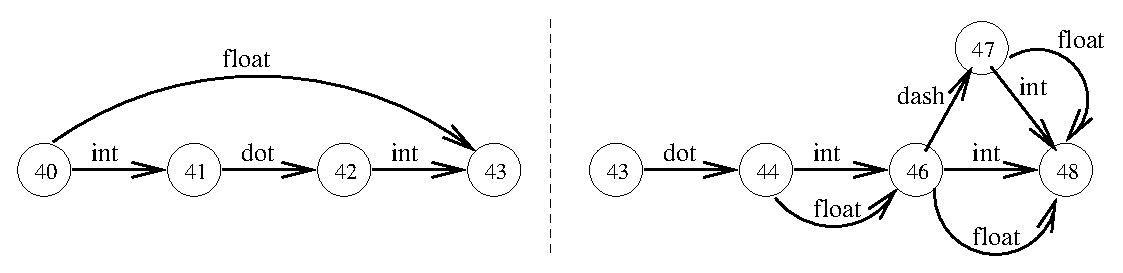
\epsfig{file=cut.eps, width=\columnwidth}
\end{center}
\caption{Cutting \seqset{} for ``2.2.13-4'' after the first float token} \label{fig:cut}
\end{figure}

Finally, the {\tt oracle} function returns the predicated structure as a ``prophecy''
along with the cut up \seqset's. 

\subsection{Format refinement with blob-finding}
The refinement phase follows the structure discovery phase to
improve the initial rough structure by applying a series of
rewriting rules. Here a new ``blob-finding'' rule is added to
the original algorithm. The purpose of this rule is to identify
``message-like'' structures in the intermediate structure and rewrite them into
a single token called {\em blob}, and thus reduce the overall complexity
of the description and increase readability. The blob-finding rule is applied
from bottom up and converts each sub-structure that is
determined to be overly complex and has a terminating pattern into a
blob. The \pads{} parser needs the terminating pattern to
know where the blob ends. Adjacent blobs are merged together. 

To determine whether a given structure is a blob, 
we compute a parameter called {\em variance} for the structure. 
It measures the total number of union/switch/enum
branches and different array lengths in the given 
structure. When the ratio between the variance and the amount of the data
this structure represents exceeds a threshold, the structure is
determined to be a possible blob. 
